\section{AlphaStar 论文解读}
 

\subsection{AlphaStar 以及背景简介} 

相比于之前的深蓝和Alpha-go,对于星际争霸2等策略对战型游戏,使用AI与人类对战难度更大。比如在星际争霸2中,操作枯燥是众所周知的,要想在玩家对战玩家(PVP)中击败对方,就得要学会各种战术,各种微操和时机。在游戏中你还得侦查对方的发展,做出正确判断进行转型,甚至要欺骗对方以达到战术目的。总而言之,想要上手这款游戏是非常困难的,但是对不起,DeepMind就做到了。

AlphaStar是DeepMind公司与暴雪使用深度强化学习技术进行计算机与星际争霸2人类玩家进行对战的产品,其在近些年在星际争霸2中打败了职业选手以及99.8\%的欧服玩家而被人所熟知。北京时间2019年1月25日凌晨2点,暴雪与谷歌DeepMind团队合作研究的星际争霸人工智能“AlphaStar”正式通过直播亮相。按照直播安排,AlphaStar与两位星际争霸2人类职业选手进行了5场比赛对决演示。加上并未在直播中演示的对决,在人类对阵AlphaStar的共计11场比赛中,人类只取得了一场胜利。DeepMind也将研究工作发表在了2019年10月的《Nature》杂志上。我们也将对于这篇论文进行深入的分析,下面是论文的链接:
\href{https://www.nature.com/articles/s41586-019-1724-z?}{Vinyals, Oriol, et al. "Grandmaster level in StarCraft II using multi-agent reinforcement learning." Nature (2019): 1-5.}

\subsection{AlphaStar 的模型输入输出是什么?——环境设计} 

构建深度强化学习模型的第一部分就是构建输入输出,对于星际争霸2这个复杂的环境,文章第一步做的就是将游戏的环境抽象成为许多的数据信息。

\subsubsection{状态(网络的输入)} 

AlphaStar将星际争霸2的环境状态分为四部分,分别为实体信息(entities)、地图信息(map)、玩家数据信息(player data)、游戏统计信息(game statistics)。

\begin{figure}[htpb]
    \centering
    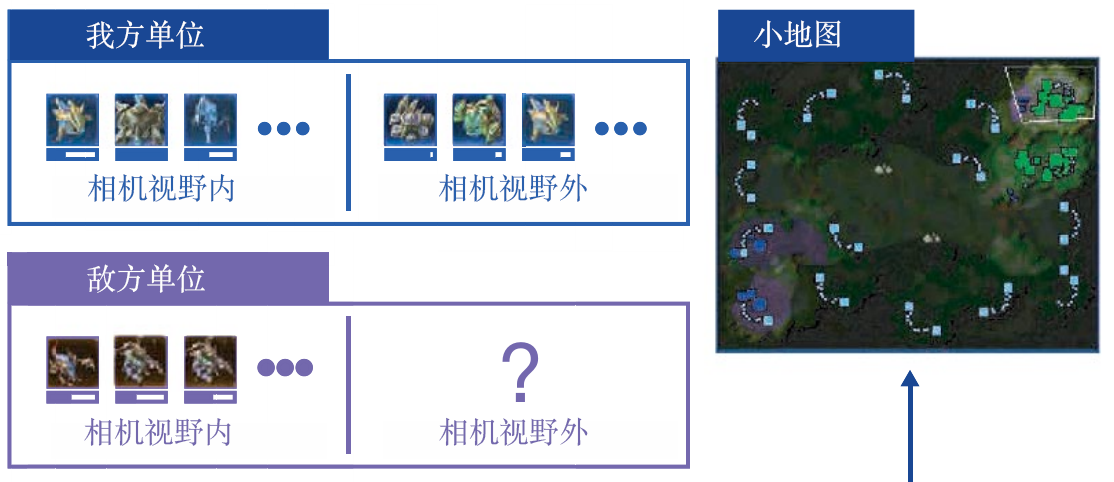
\includegraphics[width=0.7\linewidth]{res/ch13/13.1}
    \caption{}
    \label{fig:}
\end{figure}

\begin{itemize}
    \item 第一部分:实体信息,例如当前时刻环境中有什么建筑、兵种等等,并且我们将每一个实体的属性信息以向量的形式表示,例如对于一个建筑,其当前时刻的向量中包含此建筑的血量、等级、位置以及冷却时间等等信息。所以对于当前帧的全部实体信息,环境会给神经网络 $N$ 个长度为 $K$ 的向量,各表示此刻智能体能够看见的 $N$ 个实体的具体信息。(向量信息)
    \item 第二部分:地图信息,这个比较好理解,也就是将地图中的信息以矩阵的形式送入神经网络中,来表示当前状态全局地图的信息。(向量信息或者说是图像信息)
    \item 第三部分:玩家数据信息,也就是当前状态下,玩家的等级和种族等信息。(标量信息)
    \item 第四部分:游戏统计信息,视野的位置(小窗口的位置,区别于第二部分的全局地图信息),还有当前游戏的开始时间等等信息。(标量信息)
\end{itemize}

\subsubsection{动作(网络的输出)} 

AlphaStar的动作信息主要分为六个部分,分别为动作类型(Action type)、选中的单元(selected units)、目标(target)、执行动作的队列(queued)、是否重复(repeat)、延时(delay),每一个部分间是有关联的。


\begin{figure}[htpb]
    \centering
    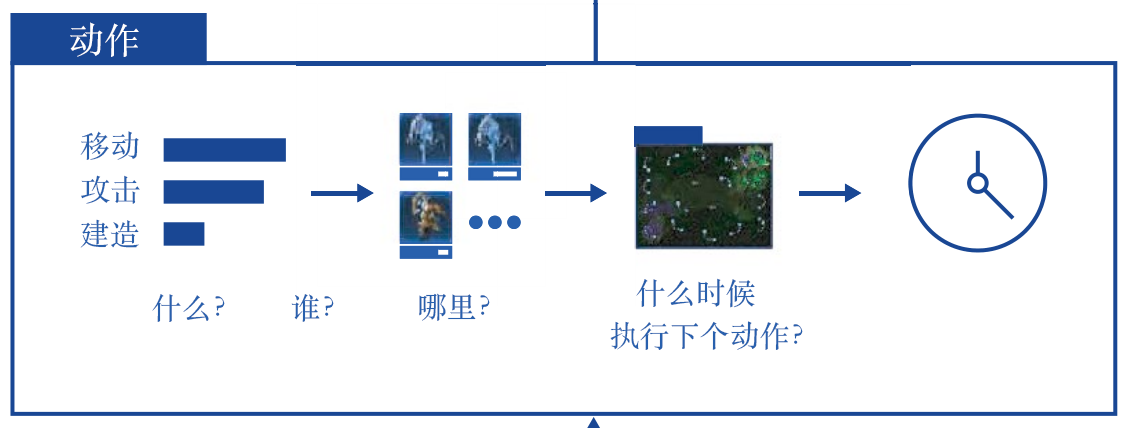
\includegraphics[width=0.7\linewidth]{res/ch13/13.2}
    \caption{}
    \label{fig:}
\end{figure}

\begin{itemize}
    \item 第一部分:动作类型,即下一次要进行的动作的类型是移动小兵、升级建筑还是移动小窗口的位置等等。
    \item 第二部分:选中的单元,即承接第一部分,例如我们要进行的动作类型是移动小兵,那么我们就应该选择具体“操作”哪一个小兵。
    \item 第三部分:目标,承接第二部分,我们操作小兵A后,是要去地图的某一个位置还是去攻击对手的哪一个目标等等,即选择目的地和攻击的对象。
    \item 第四部分:执行动作的队列,具体说是是否立即执行动作,对于小兵A,我们是到达目的地后直接进行攻击还是等待。
    \item 第五部分:是否重复做动作,如果需要小兵A持续攻击,那么就不需要再通过网络计算得到下一个的动作了,直接重复以上一个动作的相同的动作即可。
    \item 第六部分:延时,也就是等候多久才接收网络的输入,可以理解为我们人类玩家的一个操作的延迟等等。
\end{itemize}


\subsection{AlphaStar 的计算模型是什么呢?——网络结构} 

上面我们说明了AlphaStar网络的输入和输出,即状态和动作,那么从状态怎么得到动作呢?其网络结构是怎么样的呢?

\begin{figure}[htpb]
    \centering
    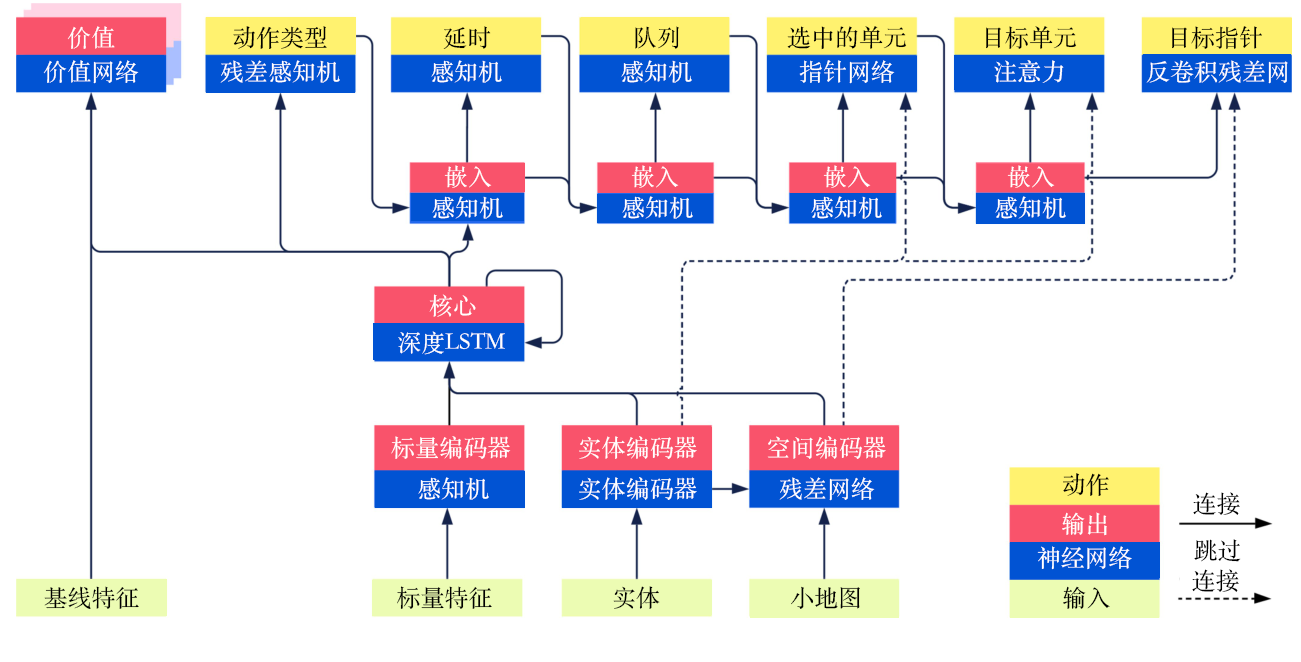
\includegraphics[width=0.7\linewidth]{res/ch13/13.3}
    \caption{}
    \label{fig:}
\end{figure}

\subsubsection{输入部分} 

\begin{figure}[htpb]
    \centering
    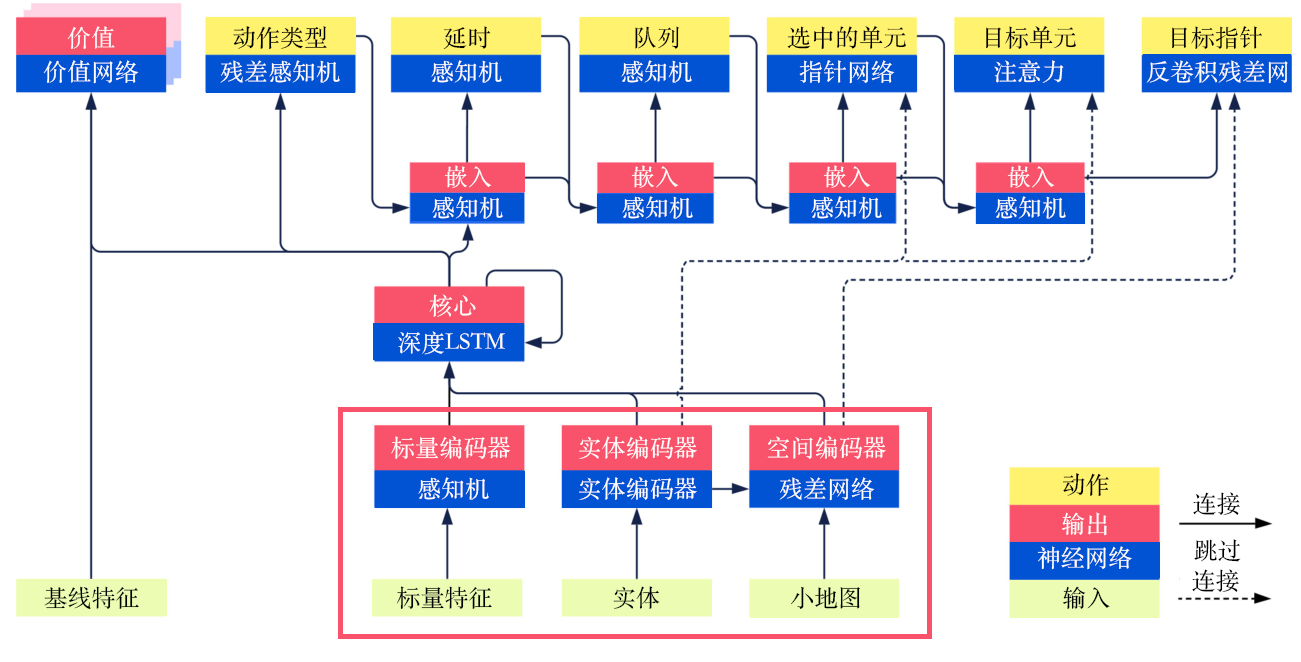
\includegraphics[width=0.7\linewidth]{res/ch13/13.4}
    \caption{}
    \label{fig:}
\end{figure}

从上图的红框可以看出,模型的输入框架中主要有三个部分,即标量特征(scalar features),例如前面叙述的玩家的等级、小窗口的位置等等信息、实体(entities),是向量即前面所叙述的一个建筑一个兵的当前的所有属性信息、小地图(minimap),即上面说的图像的数据。

\begin{itemize}
    \item 对于标量特征,使用多层感知器(MLP),就可以得到对应的向量,或者说是一个嵌入的过程。
    \item 对于实体,使用自然语言处理中常用的transformer架构作为编码器(encoder)。
    \item 对于小地图,使用图像中常用的Resnet架构作为编码器,得到一个定长的向量。
\end{itemize}

\subsubsection{中间过程} 

中间过程比较简单,即通过一个深度长短期记忆网络模块进行融合三种当前状态下的嵌入进行下一时刻的输出,并且将该结果分别送入价值网络(valueNetwork)、残差多层感知器(residual MLP)以及动作类别(actoin type)的后续的多层感知器中。

\begin{figure}[htpb]
    \centering
    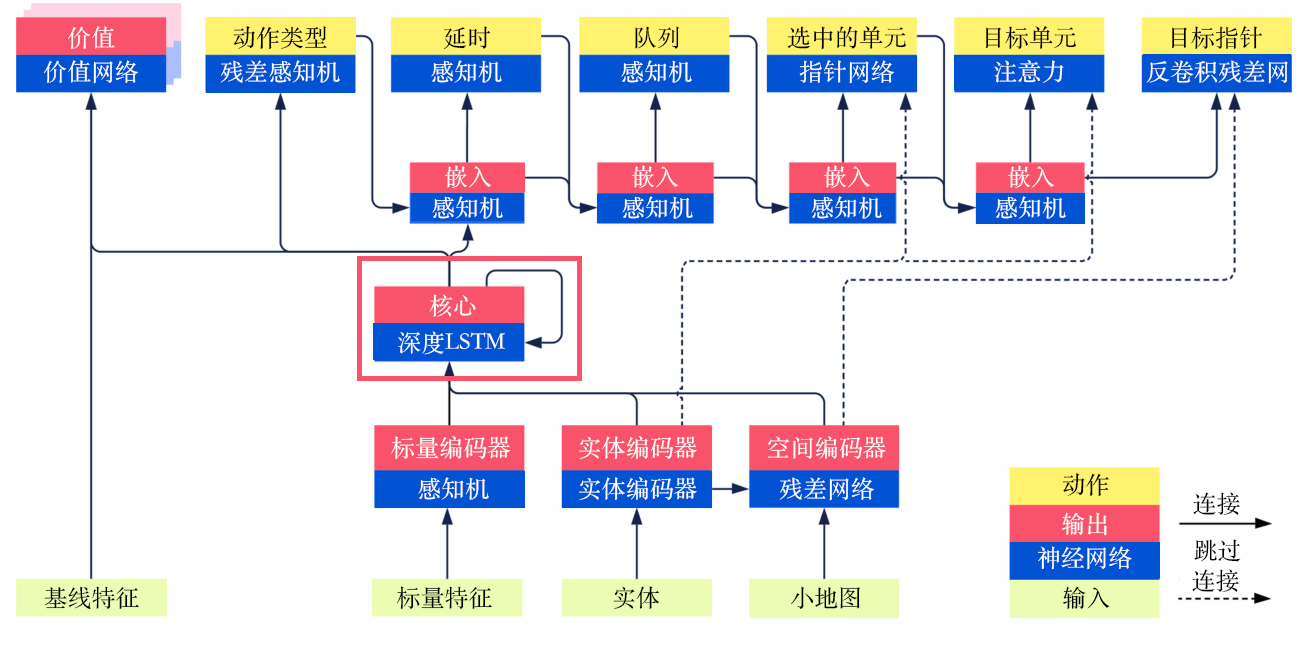
\includegraphics[width=0.7\linewidth]{res/ch13/13.5}
    \caption{}
    \label{fig:}
\end{figure}

\subsubsection{输出部分} 

正如前面介绍的,输出的动作是前后有关联的,按照顺序

\begin{figure}[htpb]
    \centering
    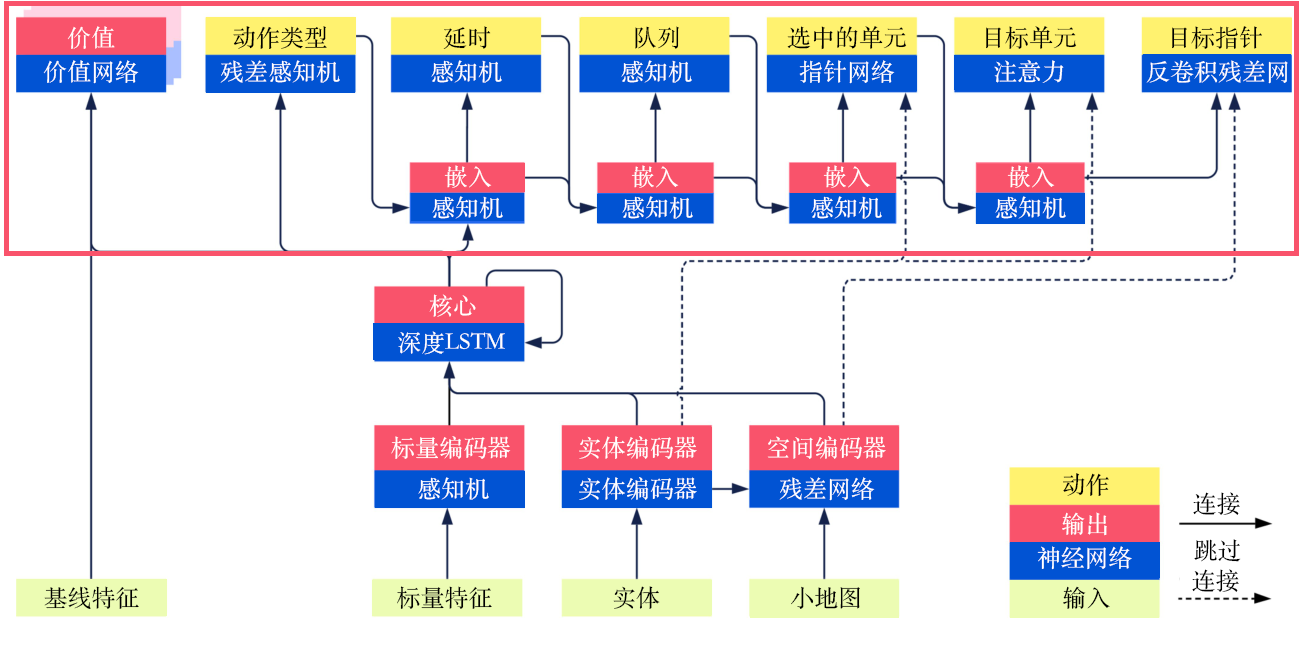
\includegraphics[width=0.7\linewidth]{res/ch13/13.6}
    \caption{}
    \label{fig:}
\end{figure}

\begin{itemize}
    \item 首先是动作类型(action type):使用深度长短期记忆网络的嵌入向量作为输入,使用残差多层感知器(residual MLP)得到动作类型(action type)的softmax激活函数的输出结果,并传给下一个子模型进行嵌入。
    \item 然后是延时(delay):使用上一个上面的嵌入的结果以及深度长短期记忆网络的结果一起输入多层感知器(MLP)后得到结果,并传给下一个子模型进行嵌入。
    \item 接下来是执行动作的队列(queued):使用延时的结果以及嵌入的结果一起输入多层感知器后得到结果,并传给下一个子模型进行嵌入。
    \item 然后是选中的单元(selected units):使用队列的结果、嵌入的结果以及实体编码后的全部结果(非平均的结果)一起送入到指针网络(pointer network)中得到结果,并传给下一个子模型进行嵌入。这里的指针网络(pointer Netowrk),即输入的是一个序列,输出是另外一个序列,并且,输出序列的元素来源于输入的序列,主要用于自然语言处理中,在这里很适合与我们的选定部分的计算。
    \item 接着是目标单元(target unit)和目标区域(target point)两者二选一进行,对于目标单元,使用注意力(attention)机制得到最优的动作作用的一个对象,对于目标区域,使用反卷积神经网络,将嵌入的向量,反卷积为地图的大小,从而执行目标移动到某一点的对应的动作。
\end{itemize}

\subsection{庞大的 AlphaStar 如何训练呢?——学习算法} 

对于上面复杂的模型,AlphaStar 究竟如何来进行训练呢?总结下来一共分为4个部分,即监督学习(主要是解决训练的初始化问题)、强化学习、模仿学习(配合强化学习)以及多智能体学习和自学习(面向对战的具体问题),下面我们一一分析:

\subsubsection{监督学习}

在训练一开始首先使用监督学习利用人类的数据进行一个比较好的初始化。模型的输入是收集到的人类的对局的信息,输出是训练好的神经网络。具体的做法是,对于收集到了人类的对局数据,在对于每一个时刻解码游戏的状态,将每一时刻的状态送入网络中得到以上每一个动作的概率分布,最终计算模型的输出以及人类数据的KL损失,并以此进行网络的优化,其中在KL损失中需要使用不同的损失函数,例如,动作类型的输出,即分类问题的损失就需要使用交叉熵(cross entropy)。而对于目标定位等类似于回归问题的就需要计算均方误差(MSE)。当然还有一些细节,大家可以自行阅读论文。总之,经过监督学习,我们的模型输出的概率分布就可以与人类玩家输出的概率分布类似。

\subsubsection{强化学习} 

这里的目标就是通过优化策略使得期望的奖励最大,即

$$
J(\pi_{\theta}) = E_{\pi_{\theta}} \sum_{t=0}r(s_t,a_t)
$$

但AlphaStar的训练的模型使用不是采样的模型,即免策略的模型,这是因为其使用的架构为类似于IMPALA的结构,即演员负责与环境交互并采样,学习者负责优化网络并更新参数,而演员和学习者通常是异步进行计算的,并且由于前面介绍的输出的动作的类型空间复杂,所以导致我们的价值函数的拟合比较困难。

这里AlphaStar利用了以下的方式进行强化学习模型的构建:
\begin{itemize}
    \item 首先是采取了经典的演员-评论员(actor-critic)的结构,使用策略网络给出当前状态下的智能体的动作,即计算 $\pi(a_t|s_t)$ ,使用价值网络计算当前状态下的智能体的期望奖励,即计算 $V(s_t) = E \sum_{t'=t}r_{t'} = E_{a_t}[r(s_t,a_t)+V(s_{t+1})]$。具体的计算方法是:
    \begin{itemize}
        \item 对于当前的状态 $s$ ,计算当前计算出的动作 $a$ 相对于“平均动作”所能额外获得的奖励。$A(s_t,a_t)=[r(s_t,a_t)+V(s_{t+1})]-V(s_t)$,即当前动作的预期奖励减去当前状态的预期奖励。在AlphaStar中,向上移动的策略更新(upgoing policy update,UPGO)也得到了应用,UPGO使用了一个迭代变量 $G_t$ 来取代原来的动作预期奖励的 $r(s_t,a_t)+V(s_{t+1})$ ,即把未来乐观的信息纳入到我们额外奖励中,上式可改写为:

        $$
        A(s_t,a_t)=G_t-V(s_t)
        $$
        
        $$
        G_t=\left\{
        \begin{aligned}
        r_t+G_{t+1} && Q(s_{s+1},a_{t+1})\geq V(s_{t+1}) \\
        r_t+V(s_{t+1}) && otherwise \\
        \end{aligned}
        \right.
        $$
    \end{itemize}
\item 在基于上面计算得到的动作,更新策略梯度,即 $\nabla_{\theta}J = A(s_t,a_t)\nabla_{\theta}log \pi_{\theta}(a_t|s_t)$,在我们之前的笔记中也介绍了,如果基于 $\pi_{\theta}$ 的分布不好求解,或者说学习策略 $\pi_{\theta}$ 与采集策略 $\pi_{\mu}$ 不同,我们需要使用重要性采样的方法,即 $\nabla_{\theta}J = E_{\pi_{\mu}}\frac{\pi_{\theta} (a_t|s_t)}{\pi_{\mu} (a_t|s_t)} A^{\pi_{\theta}}(s_t,a_t)\nabla_{\theta}log \pi_{\theta}(a_t|s_t)$。当然我们还需防止 $\frac{\pi_{\theta} (a_t|s_t)}{\pi_{\mu} (a_t|s_t)}$ 出现无穷大的情况,我们需要使用V-trace限制重要性系数。这也是用于免策略的一个更新方法,在 IMPALA 论文中的4.1小节有所体现。即将重要性系数的最大值限制为1,公式可表达如下:

$$
\nabla_{\theta}J = E_{\pi_{\mu}}\rho_tA^{\pi_{\theta}}(s_t,a_t)\nabla_{\theta}log \pi_{\theta}(a_t|s_t)
$$

$$
\rho_t = min(\frac{\pi_{\theta} (a_t|s_t)}{\pi_{\mu} (a_t|s_t)},1)
$$
\item 利用了时序差分 ($\lambda$) 来优化价值网络,并同时输入对手的数据。对于我们的价值函数 
$$
V^{\pi_{\theta}}(s_t)=E_{\pi_{\theta}}\sum_{t'=t}\gamma^{t'-t}r(s_t,a_t)=E_{a_t\sim\pi_{\theta}(\cdot|s_t)}[r(s_t,a_t)+\gamma V(s_{t+1})]
$$
,可以使用TD的方法计算均方差损失,有如下几种:
\begin{itemize}
    \item $TD(0)$ ,表达式为 $L = [(r_t+\gamma V_{t+1})-V_t]^2$ ,即当前步(step)的信息,有偏小方差
    \item $TD(1)$也就是蒙特卡洛方法,表达式为 $L = [(\sum_{t'=t}^\infty\gamma^{t'-t}r_{t'})-V_t]^2$,即未来无穷步的信息,无偏大方差
    \item $TD(\lambda)$ ,以上两个方法的加权平均。即平衡当前步、下一步到无穷步后的结果
    \begin{itemize}
        \item 已知对于 $\lambda \in (0,1)$, $(1-\lambda)+(1-\lambda)\lambda+(1-\lambda)\lambda ^2+...=1$
        \item $r_t = \lim_{T\rightarrow\infty} (1-\lambda)(r_t+V_{t+1})+(1-\lambda)\lambda(r_t+\gamma r_{t+1}+\gamma^2 V_{t+2})+...$
    \end{itemize}
    
\end{itemize}
\end{itemize}
 
\subsubsection{模仿学习} 
使用模仿学习额外引入了监督学习损失以及人类的统计量 $Z$ ,即对于建造顺序(build order)、建造单元(build Units)、升级(upgrades)、技能(effects)等信息进行了奖励。对于统计量 $Z$ ,本质来说是一系列的数据,将其作为输入信息输入到策略网络和价值网络中。另外对于人类信息的利用还体现在前面介绍的使用监督学习进行网络的预训练工作。

\subsubsection{多智能体学习/自学习} 

自学习在AlphaGo中得到了应用也就是自己和自己玩,Alpha对此做了一些更新,即有优先级的虚拟自学习策略,对于虚拟自学习就是在训练过程中,每一些时间就进行存档,并随机均匀地从存档中选出对手与正在训练的智能体对战。而有优先级的虚拟自学习指的是优先挑选能击败我的或者说常能打败智能体的对手进行训练对战,评判指标就是概率。对于AlphaStar中,其训练的智能体分为了三种,

\begin{itemize}
    \item 主智能体(main agent),即正在训练的智能体及其祖先;其中有50\%的概率从联盟中的所有人中挑选,使用有优先级的虚拟自学习策略,即能打败我的概率高,不能打败我的概率低,有35\%的概率与自己对战,有15\%的概率与能打败我的联盟利用者或者老的主智能体对战,通过利用了有优先级的虚拟自学习策略。
    \item 联盟利用者(league exploiter):能打败联盟中的所有智能体;其按照有优先级的虚拟自学习策略计算的概率与全联盟的对手训练,在以70\%的胜率打败所有的智能体或者距离上次存档 $2 \times10^9$ 步后就保存,并且在存档的时候,有25\%概率把场上的联盟利用者的策略重设成监督学习给出的初始化。
    \item 主利用者(main exploiter):能打败训练中的所有智能体,在训练的过程中,随机从3个中挑1个主智能体,如果可以以高于10\%的概率打败该智能体就与其进行训练,如果不能就从其他的老主智能体中再挑选对手,当以70\%的胜率打败全部三个正在学习的策略主智能体,或者距上次存档 $4 \times10^9 $ 个步之后就存,并且进行重设初始化的操作。
\end{itemize}


他们的区别在于:
\begin{itemize}
    \item 如何选取训练过程中对战的对象;
    \item 在什么情况下存档(snapshot)现在的策略;
    \item 以多大的概率将策略的参数重设为监督训练给出的初始化。
\end{itemize}


\subsection{AlphaStar实验结果如何呢?——实验结果} 

\subsubsection{宏观结果} 

\begin{figure}[htpb]
    \centering
    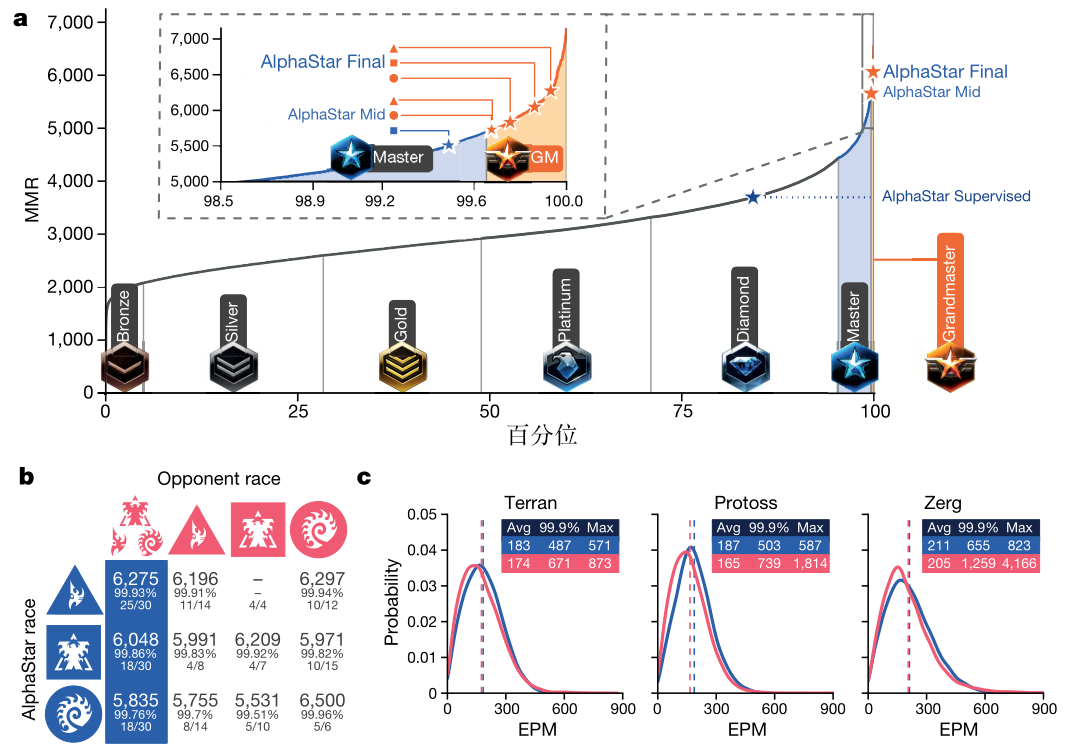
\includegraphics[width=0.5\linewidth]{res/ch13/13.7}
    \caption{}
    \label{fig:}
\end{figure}

图A为训练后的智能体与人类对战的结果(天梯图),具体地,刚刚结束监督学习后的AlphaStar可以达到钻石级别,而训练到一半(20天)以及训练完结(40天)的AlphaStar可以达到大师的级别。AlphaStar已经可以击败绝大多数的普通玩家。

图B为不同种族间对战的胜率。

图C为《星际争霸II》报告的每分钟有效行动分布情况(EPM),其中蓝色为AlphaStar最终的结果,红色为人类选手的结果虚线显示平均值。

\subsubsection{其他实验(消融实验)} 

AlphaStar的论文中也使用了消融实验,即控制变量法,来进一步分析每一个约束条件对于对战结果的影响。下面举一个特别的例子:

\begin{figure}[htpb]
    \centering
    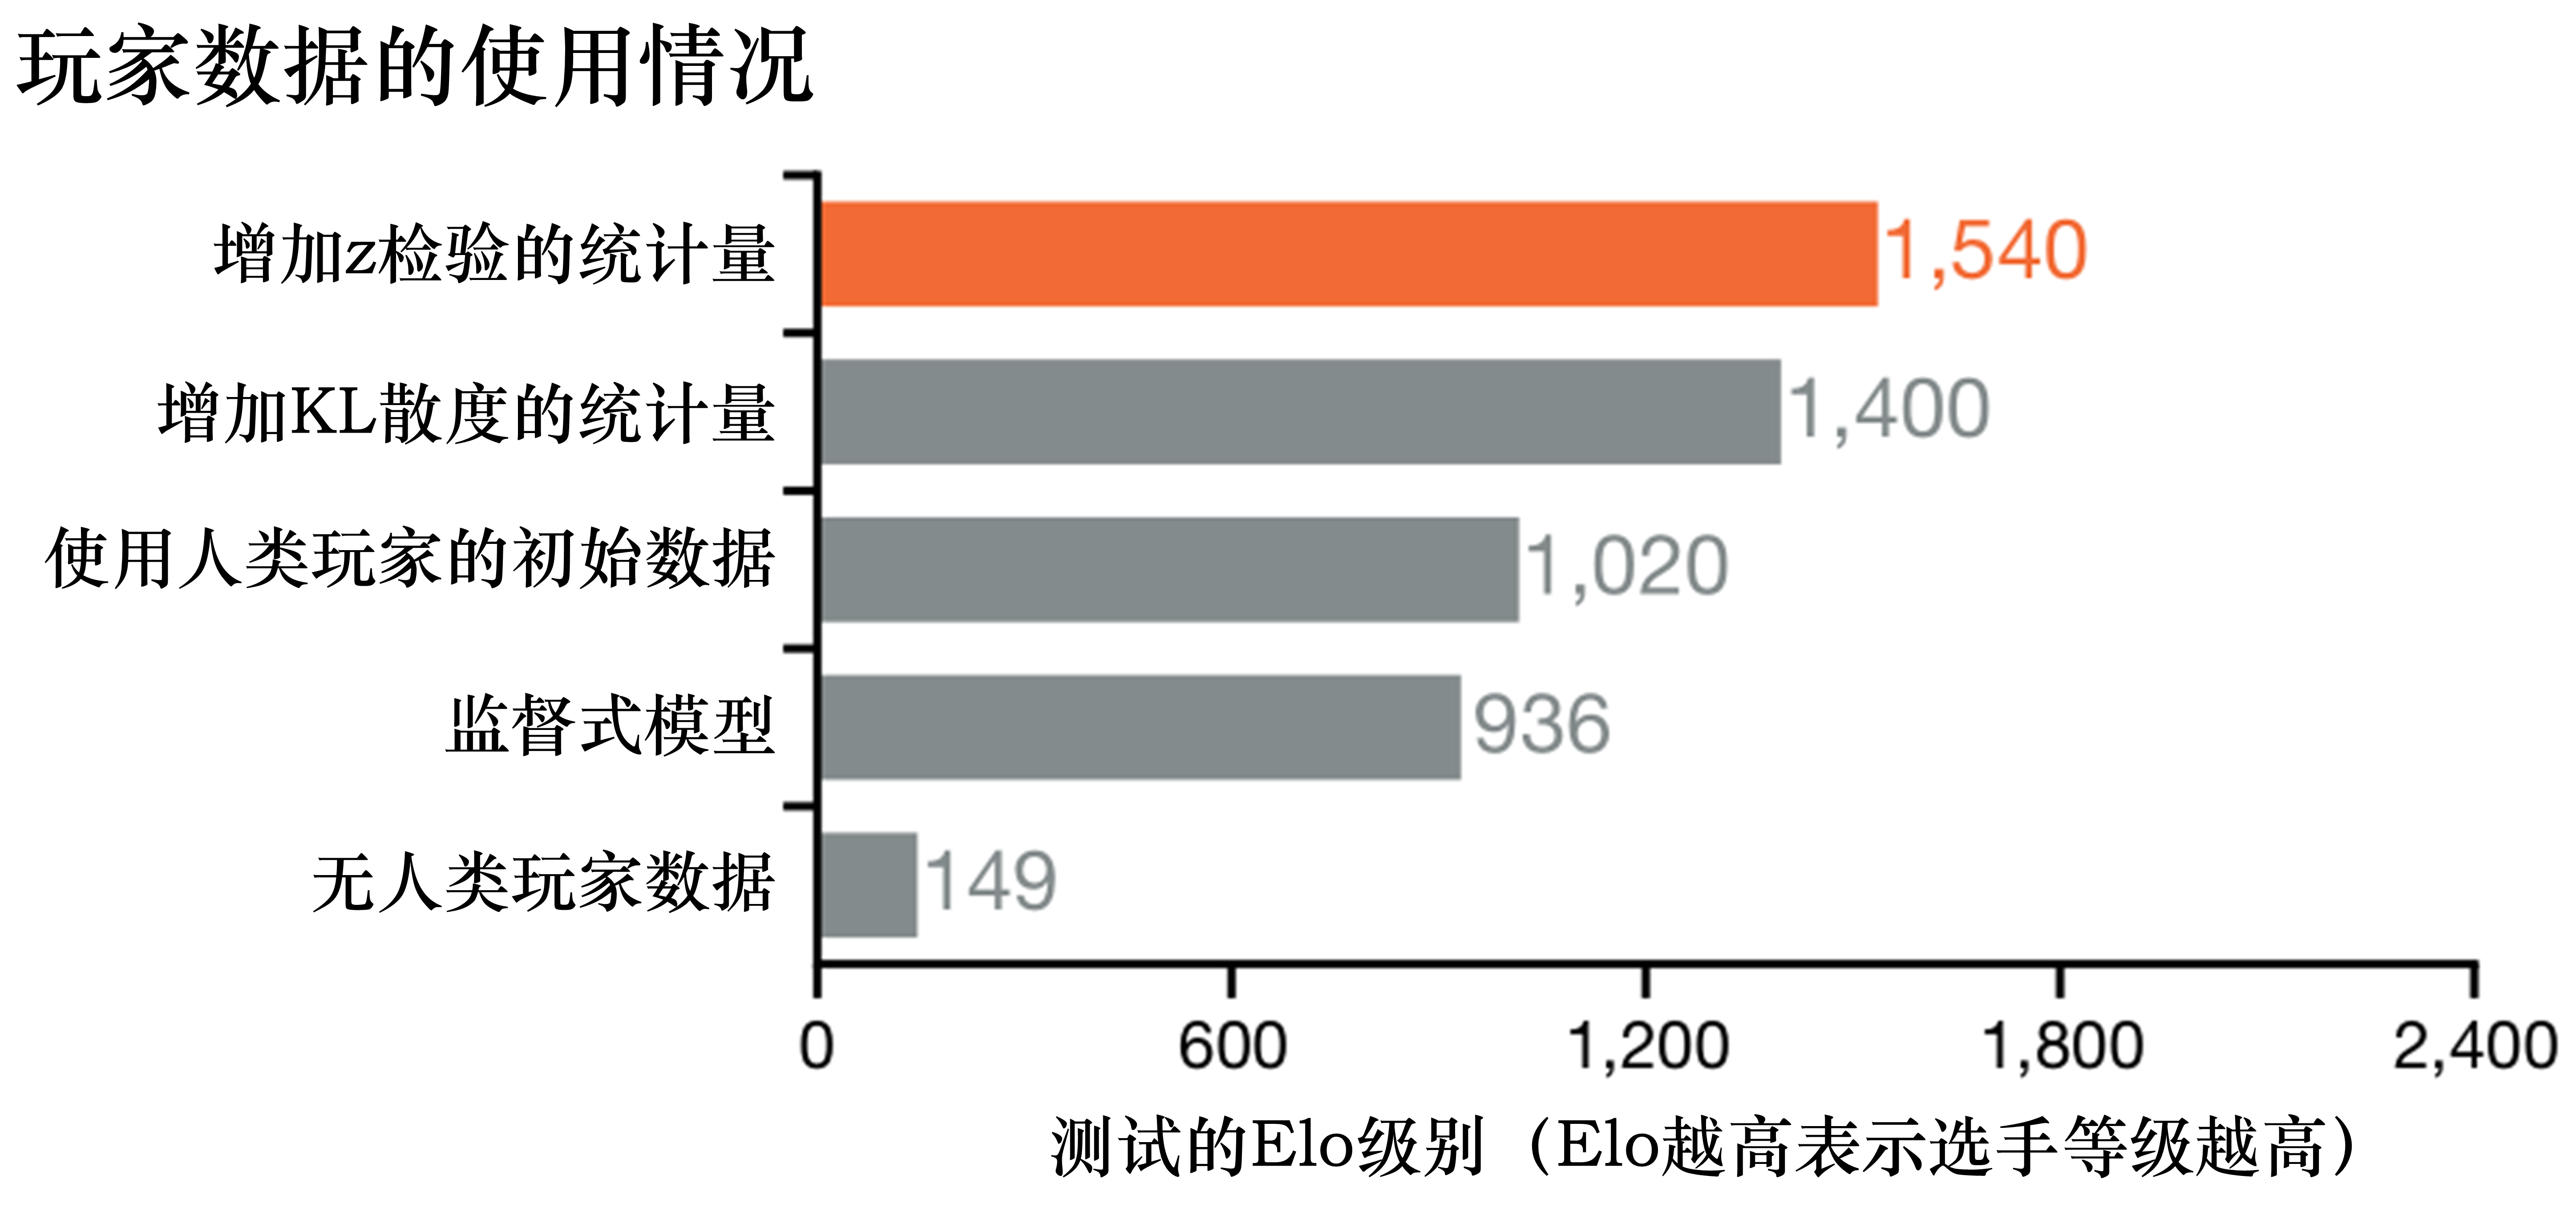
\includegraphics[width=0.5\linewidth]{res/ch13/13.8}
    \caption{}
    \label{fig:}
\end{figure}

上面的图片表示的是人类对局数据的使用的情况。可以看到如果没有人类对局数据的情况下,数值仅仅为149,但是只要经过了简单的监督学习,对应的数值就可以达到936,当然使用人类初始化后的强化学习可以达到更好的效果,利用强化学习加监督学习的KL损失可以达到接近于完整的利用人类统计量 $Z$ 的效果。可以分析出,AlphaStar中人类对局的数据对于整个模型的表现是很重要的,其并没有完全像AlphaGo一样,可以不使用人类数据的情况。

\subsection{关于 AlphaStar 的总结} 

\subsubsection{总结} 
\begin{itemize}
    \item AlphaStar设计了一个高度可融合图像、文本、标量等信息的神经网络架构,并且对于网络设计使用了自回归(autoregressive)从而解耦了结构化的动作空间;
    \item 模仿学习和监督学习的内容,例如人类统计量 $Z$ 的计算方法;
    \item 复杂的深度强化学习方法以及超复杂的训练策略;
    \item 当然了,大量的计算资源,对于此,原文表述如下:每个智能体使用32个第三代张量处理单元(TPUs 23)进行了44天的训练。在训练期间,创建了近900个不同的游戏玩家。
\end{itemize}



